%%% LaTeX Template based on the Project Report 
%%% Found on http://www.howtotex.com/

%%% Preamble
\documentclass[paper=a4, fontsize=11pt]{scrartcl}
\usepackage[T1]{fontenc}
\usepackage{fourier}

\usepackage[english]{babel}	% English language/hyphenation
\usepackage[protrusion=true,expansion=true]{microtype}% Better typography

\usepackage{amsmath,amsfonts,amsthm}	% Math packages
\usepackage[pdftex]{graphicx}% Enable pdflatex
\usepackage{url}
\usepackage{listings}
\usepackage[hang, small,labelfont=bf,up,textfont=it,up]{caption} % Custom captions under/above floats
\usepackage{booktabs}% Nicer tables


%%% Custom sectioning (sectsty package)
\usepackage{sectsty}% Custom sectioning (see below)
\allsectionsfont{\normalfont\scshape}% Change font of al section commands


%%% Custom headers/footers (fancyhdr package)
\usepackage{fancyhdr}
\pagestyle{fancyplain}
\usepackage{lastpage}
\fancyhead{}% No page header
\fancyfoot[L]{\small Last Name}% You may remove/edit this line 
\fancyfoot[C]{\small Assignment 3}
\fancyfoot[R]{\thepage~ of ~\pageref{LastPage}}% Pagenumbering
\renewcommand{\headrulewidth}{0pt}% Remove header underlines
\renewcommand{\footrulewidth}{0pt}% Remove footer underlines
\setlength{\headheight}{13.6pt}

\title{
		\usefont{OT1}{bch}{b}{n}
		\normalfont \Large Robot Manipulation \\
		\huge Assignment 1 \\ % Update to the current assignment
}

\author{\normalfont \normalsize Firstname Lastname % Write your name
		\\[-3pt] }
\date{\normalsize \today}


\begin{document}
\maketitle

 
\section{Summary}
The summary is meant to prepare you for the exam. Make notes as you would use them for studying and use your own words. 
\begin{itemize}
	\item Some important point
	\item And relevant notes
\end{itemize}

\section{This week's topic}

The purpose of the homework is to make us see how well you have grasped the concepts. You should always include all the steps on how you arrived at your answers on any homework.
Your solutions must be self-contained. All arguments, theorems, equations, etc., behind your answers as well as their procedures have to be contained within your homework.
Even if you use any external tools, remember that your submission must contain all the relevant (mathematical/conceptual) steps and explanations!  

Don't forget to include the instruction text of the questions.

\begin{enumerate}
	\item First question
	
	Answer containing all the steps. Remember that you can include the drawings by hand, as long as they are properly scanned. Use \LaTeX ~to properly reference them. 
	\begin{figure}[h]
		\label{fig:frame}
		\begin{center}
			\caption{An example reference frame. \\ Include the file name and scale the images accordingly.}
			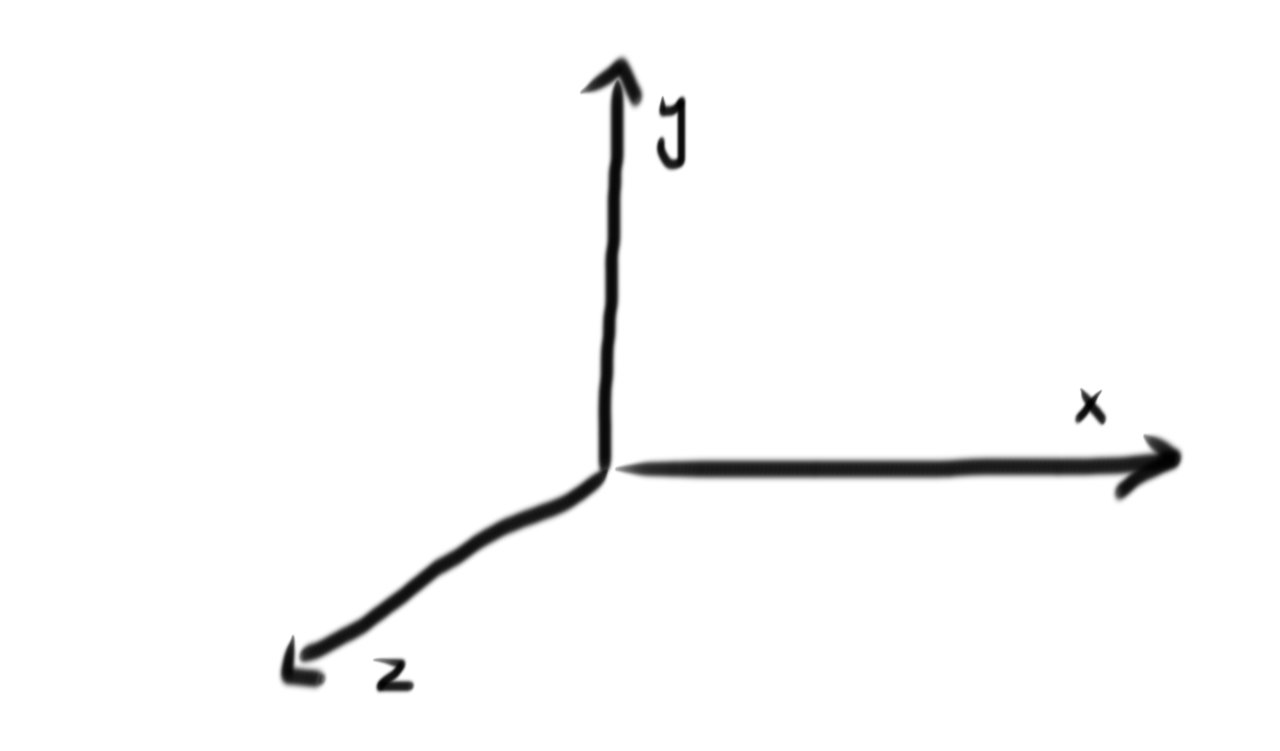
\includegraphics[width=.3\textwidth]{images/Frame}
		\end{center}	
	\end{figure}
	
	\item Include the relevant snippets of your code in your answer. 
	Include your working code with a README on how to run it in the zipped file of your assignment. Your code must be properly commented and your variable names must make sense.
	 
	In this case, the template header is relevant only to show you the minimal information you should include. Don't forget to include your data (and your teammate's) in any file you submit.
	\lstinputlisting[language=Python, numbers=left, firstline=1, 
				lastline=15, frame=L, title=\lstname]{code/example.py}
	
	\item This basic example only shows the relevant lines of code.
	\lstinputlisting[language=Python, numbers=left, firstline=10, 
				lastline=18, frame=L, title=\lstname]{code/transform.py}

\end{enumerate}

\textbf{\Large Don't forget to cite the relevant books \cite{craig2005}, articles, tutorials or other materials that you used.}

\bibliography{references}
\bibliographystyle{unsrt}

\end{document}